\documentclass[11pt,a4aper]{article}
\pdfoutput=1

\usepackage[utf8]{inputenc}
%\usepackage{polski}
\usepackage[lf,enc=t1]{berenis}
%\usepackage[main=english,polish]{babel}

\renewcommand{\baselinestretch}{1}
\usepackage[UKenglish]{isodate}
\cleanlookdateon

%%%%% Fonts, symbols, colours, microtypography
\usepackage{amsfonts,amsmath,amssymb,amsthm,mathtools,microtype} % Symbols &microtypography
\usepackage[dvipsnames]{xcolor} % Colours with names -- see https://www.overleaf.com/learn/latex/Using_colours_in_LaTeX for list
\usepackage[noBBpl]{mathpazo} % Palatino, but not for mathbb

%%%%% Figures, tables, lists
\usepackage[labelsep=period,labelfont=bf,justification=centering]{caption}
\usepackage{float,graphicx,subcaption}
\usepackage{enumitem}
\setlist[itemize]{topsep=0ex,itemsep=0ex,parsep=0.4ex}
\setlist[enumerate]{topsep=0ex,itemsep=0ex,parsep=0.4ex}

\usepackage{parskip,fullpage}
\usepackage{thm-restate}
\usepackage[textsize=scriptsize]{todonotes}
\setlength{\marginparwidth}{2cm}%to have larger todonotes
\usepackage{comment}

\usepackage{array}
\usepackage{ifthen}

%%%%% Hyperlinking
\usepackage[hyphens]{url} % Urls together with line breaking them
\usepackage[linktoc=all,hidelinks,colorlinks,unicode=true]{hyperref} % Must be loaded after url
\usepackage[capitalise,compress,nameinlink,noabbrev]{cleveref} % Must be loaded after hyperref
\hypersetup{linkcolor={blue!70!black},citecolor={black},urlcolor={blue!70!black}}
\usepackage{hyperref}

\usepackage{listings}
\definecolor{codegreen}{rgb}{0,0.6,0}
\definecolor{codegray}{rgb}{0.5,0.5,0.5}
\definecolor{codepurple}{rgb}{0.58,0,0.82}
\lstdefinestyle{mystyle}{
    backgroundcolor=\color{white},   
    commentstyle=\color{codegreen},
    keywordstyle=\color{magenta},
    numberstyle=\tiny\color{codegray},
    stringstyle=\color{codepurple},
    basicstyle=\ttfamily\footnotesize,
    breakatwhitespace=false,         
    breaklines=true,                 
    captionpos=b,                    
    keepspaces=true,                 
    numbers=left,                    
    numbersep=5pt,                  
    showspaces=false,                
    showstringspaces=false,
    showtabs=false,                  
    tabsize=2
}
\lstset{style=mystyle}


\usepackage{tikz}
\usetikzlibrary{decorations.markings}
\tikzstyle{classic}=[draw=black,fill = black,inner sep = 1pt,circle]

\newtheorem{theorem}{Theorem}
\newtheorem{lemma}[theorem]{Lemma}
\newtheorem{claim}[theorem]{Claim}
\newtheorem*{claim*}{Claim}
\newtheorem{conjecture}[theorem]{Conjecture}
\newtheorem{corollary}[theorem]{Corollary}
\newtheorem{question}[theorem]{Question}
% \theoremstyle{definition}
\newtheorem{remark}[theorem]{Remark}
\newtheorem{problem}[theorem]{Problem}

\makeatletter
\def\namedlabel#1#2{\begingroup
   \def\@currentlabel{#2}%
   \label{#1}\endgroup
}
\makeatother

\newenvironment{poc}{\begin{proof}[Proof of
    Claim]\renewcommand*{\qedsymbol}{$\blacksquare$}}{\end{proof}}

\newenvironment{csproblem}[1]{\textsc{#1}:\\}{}


\crefname{subsection}{Subsection}{Subsections}

%%%%% Renew commands

\renewcommand{\ge}{\geqslant}
\renewcommand{\le}{\leqslant}
\renewcommand{\geq}{\geqslant}
\renewcommand{\leq}{\leqslant}
% \renewcommand{\eps}{\varepsilon}
\renewcommand{\emptyset}{\varnothing}

%%%%% mathbold and mathcal
\newcommand*{\eps}{\varepsilon}
\renewcommand{\phi}{\varphi}
\newcommand*{\bE}{\mathbb{E}}
\newcommand*{\bN}{\mathbb{N}}
\newcommand*{\bP}{\mathbb{P}}
\newcommand*{\bR}{\mathbb{R}}
\newcommand*{\bZ}{\mathbb{Z}}
\newcommand*{\cF}{\mathcal{F}}
\newcommand*{\cO}{\mathcal{O}}
\newcommand*{\cE}{\mathcal{E}}
\newcommand*{\cI}{\mathcal{I}}
\newcommand*{\cJ}{\mathcal{J}}
\newcommand*{\cR}{\mathcal{R}}
\newcommand*{\cC}{\mathcal{C}}
\newcommand*{\cX}{\mathcal{X}}
\newcommand*{\cG}{\mathcal{G}}
\newcommand*{\cY}{\mathcal{Y}}
\newcommand*{\cB}{\mathcal{B}}
\newcommand*{\cS}{\mathcal{S}}
\newcommand*{\cD}{\mathcal{D}}
\newcommand*{\cM}{\mathcal{M}}
\newcommand*{\cP}{\mathcal{P}}
\newcommand*{\cQ}{\mathcal{Q}}
\newcommand*{\cA}{\mathcal{A}}
\newcommand*{\cU}{\mathcal{U}}
\DeclareMathOperator{\sq}{\square}

\DeclarePairedDelimiter{\set}{\{}{\}}
\DeclarePairedDelimiter{\abs}{\lvert}{\rvert}
\DeclarePairedDelimiter{\floor}{\lfloor}{\rfloor}
\DeclarePairedDelimiter{\ceil}{\lceil}{\rceil}

% Colors
\newcommand{\colora}{Goldenrod}
\newcommand{\colorb}{SkyBlue}
\newcommand{\colorc}{Sepia}
\newcommand{\colord}{orange}
\newcommand{\colore}{MidnightBlue}
\newcommand{\colorf}{white}
\newcommand{\colorg}{black}

\newcommand{\cola}{\coloredbullet{\colora}}
\newcommand{\colb}{\coloredbullet{\colorb}}
\newcommand{\colc}{\coloredbullet{\colorc}}
\newcommand{\cold}{\coloredbullet{\colord}}
\newcommand{\cole}{\coloredbullet{\colore}}
\newcommand{\colf}{\coloredbullet{\colorf}}
\newcommand{\colg}{\coloredbullet{\colorg}}

\definecolor{color1}{rgb}{.8,.1,.1}
\definecolor{color2}{rgb}{.1,.8,.1}
\definecolor{color3}{rgb}{.1,.1,.8}

  
%%% Comments
\newcommand{\bartosz}[1]{{\color{blue} BW: #1}}
\newcommand{\clement}[1]{{\color{orange} CL: #1}}
\newcommand{\nicolas}[1]{{\color{purple} UG: #1}}
\newcommand{\ugo}[1]{{\color{red} NT: #1}}

\title{Shift graph recognition is NP-complete}

\date{\today}

\author{
Bartosz Walczak\footnotemark[1] \and 
Cl\'ement Legrand-Duchesne\footnotemark[1]\and
Ugo Giocanti\footnotemark[1] \and
Nicolas Trotignon\footnotemark[2]
}

\begin{document}
\maketitle

\renewcommand{\thefootnote}{\fnsymbol{footnote}} % Make affiliation marks symbols

\footnotetext[1]{Theoretical Computer Science Department, Faculty of Mathematics and Computer Science, Jagiellonian University, Kraków, Poland.}
\footnotetext[2]{Univ Lyon, EnsL, UCBL, CNRS, LIP, F-69342, LYON Cedex 07, France}

\renewcommand{\thefootnote}{\arabic{footnote}} % Return to normal footnote symbols

\begin{abstract}
\end{abstract}

A class of graphs is \emph{hereditary} if it closed under taking induced
subgraphs.  A hereditary class $\mathcal C$ of graph is $\chi$-bounded if there
exists a function $f$ such that for all graphs $G\in \mathcal C$,
$\chi(G) \le f(\omega(G))$.  Not all hereditary classes of graphs are
$\chi$-bounded because there exist triangle-free graphs of arbitrarily large
chromatic number.  Several constructions are known and their structure attracted
some attention lately. In particular, a construction due to Burling turned out
to be a counter-example to several conjectures about algorithms in non-$\chi$
bounded classes.

In \cref{tab:complexity}, we review the simplest and most well-known
constructions of triangle-free graphs of arbitratily large chromatic number.
Note that most of these constructions (all of them except shift) are usually
obtained by generating a sequence of triangle-free graphs
$(G_k)_{k\in \mathbb{N}}$ such that $\chi(G_k) = k$ for all $k$. We turn this
into a hereditary class by considering the induced subgraphs of the graphs in
the sequence.

Three problems particularly attracted attention: recognition, maximum
independent set problem and 3-coloring. The complexity of all of them is known
for all the classes from \cref{tab:complexity} (where a reference is given),
except shift graphs. The goal of the present paper is to prove that the three
problems are NP-complete for shift graphs.
\begin{table}[h!]
  \centering
  \begin{tabular}{|l|c|c|c|}
    \hline
    Graph class & Recognition & Minimum Independent set & 3-Colouring \\
    \hline
    Mycielski & P & NPC \cite{poljak1974Note} & NPC \cite{lovasz1973Covering,maffray1996NPcompleteness} \\
    Zykov & NPC \cite{marin2024Structural} & NPC \cite{marin2024Structural} & NPC \cite{marin2024Structural} \\
    Blanche-Descartes & NPC \cite{marin2024Structural} & NPC \cite{marin2024Structural} & NPC \cite{marin2024Structural} \\
    Burling & P \cite{rzazewski2024Polynomial} & P \cite{rzazewski2024Polynomial} & NPC \cite{walczak2025Private}\\
    Twincut & P \cite{bourneuf2025Private} & NPC \cite{bourneuf2025Private} & NPC \cite{bourneuf2025Private} \\
    Shift & NPC [*] & NPC [*] & NPC [*] \\
    \hline
  \end{tabular}  
  \caption{Complexity of Recognition, Minimum independent set and 3-Colouring of
    the main constructions of triangle-free graph of large chromatic number}
  \label{tab:complexity}
\end{table}

Three problems particularly attracted attention: Recognition, Maximum
independent set problem and 3-Colouring. The complexity of all of them is known
for all the classes from \cref{tab:complexity} (where a reference is given),
except shift graphs and Kneser graphs. The goal of the present paper is to prove
that the three problems are NP-complete for shift graphs. Surprisingly, we see
from \cref{tab:complexity} that 3-Colouring is NP-complete in all known
constructions of triangle-free graphs of high chromatic number, which motivates
the following conjecture:
\begin{conjecture}
  3-Colouring is NP-complete in all hereditary graph classes of unbounded
  chormatic number.
\end{conjecture}


For most of these constructions of triangle-free graphs with high chromatic
number, there exist variants producing graphs with arbitrarily large girth or
odd-girth, and unbounded chromatic number. More precisely, shifts graphs, Zykov,
Blanche-Descartes, Twincut or Mycielski graphs with odd-girth at least $g$ have
unbounded chromatic number. We believe that the complexity results of
\cref{tab:complexity} also hold with this additional condition in these
classes. In the particular case of shift graphs, $k$-iterated shift graphs have
odd-girth at least $2k+3$ but may contain four-cycles. Each of our
NP-completeness results extends to the class of $k$-iterated shift graphs.
Moreover, we prove that shift graphs of girth at least five are 3-colourable,
but that maximum independent set is still NP-complete on shift graphs of
arbitrarily large girth.


% \paragraph{Abyssal classes}
% In \cite{abrishami2025Burling}, Abrishami et. al. prove that the class of
% Burling graph forms a minimal hereditary class of unbounded chromatic number:
% any proper hereditary subclass of Burling graph has bounded chromatic
% number. The only other known graph class with this property is cliques. At first
% view, the hereditary closures of any construction of triangle-free graphs with
% large chromatic number are natural candidates in the search for other minimal
% hereditary classes of unbounded chromatic number. However, the classes of
% Mycielski, Blanche-Descartes, Twincut, Zykov and shift graphs are not minimal.

% Indeed, Mycielski graphs are universal for triangle-free graphs, and
% Blanche-Descartes graphs (respectively Twincut graphs or shift graphs) contain
% graphs of arbitrarily large chromatic number and arbitrarily large girth
% (respectively odd girth). Thus none of these classes is
% minimal. Blanche-Descartes and Twincut graphs are special cases of Zykov graphs,
% hence Zykov graphs cannot form a minimal hereditary class of unbounded chromatic
% number.

% A class is \emph{abyssal} if it contains no minimal subclass of unbounded
% chromatic number. 


We prove in \cref{sec:MIS} that Maximum independent set (\textsc{MIS}) is
NP-complete in shift graphs. We prove in \cref{sec:3COL} that 3-Colouring
(\textsc{3-Col}) is NP-complete in shift graphs and in \cref{sec:recognition}
that recognising shift graphs is also NP-complete.

\section{Preliminaries}

\paragraph{Notations and glossary} A digraph $D$ consists of a set $V(D)$ of
vertices and a set $A(D)$ of directed edges denoted $(u,v)$, $uv$ or $u \to v$
and called \emph{arcs}. Given an arc $a=u \to v$, the \emph{head} of $a$ is $v$
and its \emph{tail} is $u$. An oriented graph is a digraph with no opposite
arcs. The \emph{support} of a digraph $D$ is the non-directed graph $G$ obtained
by removing the orientations of the arcs of $D$, that is $V(G) = V(D)$ and
$E(G) = \{\{x,y\} \colon (x,y) \in A(D)\}$. We say that a vertex $u$ of a
digraph $D$ is \emph{transitive} if it is neither a source nor a sink. A
\emph{$k$-walk} (respectively \emph{$k$-path}) is a sequence of $k$ (distinct)
consecutive arcs. The \emph{prefix} (resp. \emph{suffix}) of length $k$ of a path $P$ are the
first (or last) $k$ arcs of $P$.

\paragraph{Line digraphs}
The \emph{line digraph} $L(D)$ of $D$ is the digraph whose vertices are the arcs
of $D$ and in which there is an arc from $a$ to $b$ if the head of $a$ is the
tail of $b$ in $D$, in other words when $a$ and $b$ are consecutive. We refer to
$D$ as a \emph{root} digraph of $L(D)$. The \emph{$k$-iterated line digraph}
$L^k(D)$ of $D$ is then defined recursively by $L^k(D) = L(L^{k-1}(D))$ and
$L^0(D) = D$.  Equivalently, the vertices of $L^k(D)$ are the directed $k$-walks
in $D$ and $L^k(D)$ contains an arc from $a$ to $b$ if the corresponding
directed walks overlap on the $k$ last vertices of $a$ and the $k$ first
vertices of $b$, namely $a = (v_0, \ldots, v_k)$ and $b=(v_1, \ldots, v_{k+1})$
with $(v_i,v_{i+1}) \in A(D)$ for all $i$.

The following result of Beineke characterises line digraphs of digraphs.
\begin{lemma}[Beineke~\cite{beineke1968Derived}]\label{lem:forbidden_config}
  A digraph $D$ is the line digraph of an oriented graph $D'$ if and only if the two
  following conditions are satisfied:
  \begin{enumerate}
  \item If $D$ contains three arcs $a$, $b$ and $c$ such that $a$ and $b$ have
    the same tail, and $b$ and $c$ have the same head, then $D$ also contains an
    arc from the tail of $c$ to the head of $a$.
  \item $D$ does not contain four arcs $a$, $b$, $c$ and $d$ such that the tails
    of $a$ and $c$ are identical, the heads of $d$ and $b$ are identical, and
    the head of $a$ (resp. $c$) is the tail of $b$ (resp. $d$).  
  \end{enumerate}
\end{lemma}
% \begin{figure}[ht]
%   \centering
%   \begin{subfigure}{.4\textwidth}
%     \centering
%     \begin{tikzpicture}
%       \node[classic] (1) at (0,0);
%       \node[classic] (2) at (1,.5);
%       \node[classic] (3) at (1,-.5);
%       \node[classic] (4) at (2,0);

%       \draw (1) -> (2);
%       \draw (1) -> (3);
%       \draw (2) -> (4);     
%     \end{tikzpicture}
%     \caption{Consistent neighbourhoods}
%     \label{sfig:config1}
%   \end{subfigure}%
%   \hfill
  
%   \begin{subfigure}{.4\textwidth}
%     \centering
%     \begin{tikzpicture}
%       \node[classic] (1) at (0,0);
%       \node[classic] (2) at (1,.5);
%       \node[classic] (3) at (1,-.5);
%       \node[classic] (4) at (2,0);

%       \draw (1) -> (2);
%       \draw (1) -> (3);
%       \draw (2) -> (4);     
%     \end{tikzpicture}
%     \caption{Forbidden configuration, Condition 2:Consistent neighbourhoods}
%     \label{sfig:config2}
%   \end{subfigure}%
%   \caption{Characterisation of orientations of line digraphs.}
%   \label{fig:config_line_digraph}
% \end{figure}
Note that the second condition forbids parallel arcs in $D'$, while the first
one ensures that the all arcs of $D'$ entering a fixed vertex have identical
out-neighbourhood in $D$. Moreover, note that these two conditions ensure that
the only allowed orientations of a triangle is the cyclic one and the only
allowed orientations of the 4-cycles of $D$ are the cyclic ones and the ones
alternating at each vertex.

Beineke's characterisation shows that line digraphs of digraphs can be
recognised in polynomial time. However, Chv\'atal and Ebenegger showed that
recognising their support is NP-complete~\cite{chvatal1990Note}.

\paragraph{Shift graphs}
% The class of $k$-shift graphs (or simply shift graphs for $k=2$) is the
% hereditary closure of the graphs $\{G_{n,k} : n \ge 1\}$, that is, all induced
% subgraph of some $G_{n,k}$. Note that this definition is equivalent to saying
% that $k$-shift graphs are the supports of the $(k-1)$-iterated line digraphs of
% all directed acyclic graphs.

The shift graph construction is the sequence of graphs $(G_n)_{n\in \mathbb{N}}$
such that $G_n$ is the graph whose vertices are the ordered pairs $(a_1,a_2)$ of
$[n]$ such that $1 \le a_1 < a_2 \le n$, in which two vertices $a = (a_1, a_2)$
and $b = (b_1, b_2)$ are adjacent if $b_1 = a_2$ (or $a_1 = b_2$). From this
definition, it is straightforward to check that $G_n$ is the support of the line
digraph of the transitive tournament on $n$ vertices.

The $k$-iterated shift graph $G_{n,k}$ (sometimes referred to as generalised
shift graph) is the graph whose vertices are ordered $(k+1)$-tuples
$(a_0, \ldots, a_k)$ of $[n]$ such that $1 \le a_0 < a_1 < \ldots, < a_k \le n$,
in which two vertices $a = (a_0, \ldots, a_k)$ and $b = (b_0, \ldots, b_k)$ are
adjacent if $b_i = a_{i+1}$ for all $i \in [k-1]$ (or $a_i = b_{i+1}$ for all
$i \in [k-1]$). From this definition, it is straightforward to check that
$G_{n,k}$ is the support of the $k$-iterated line digraph of the transitive
tournament on $n$ vertices. The graph $G_{n,k}$ has odd-girth $2k+3$, in
particular shift graphs are triangle-free.

The class of shift graphs is the hereditary closure of the graphs
$(G_n)_{n\in \mathbb{N}}$, that is, all induced subgraph of some $G_n$. Note that this
definition is equivalent to saying that shift graphs are the supports of the
line digraphs of all directed acyclic graphs. Equivalently,
shift graphs are often defined by their interval representation and the natural
acyclic orientation that arises from it: the vertices of a shift graph are
indexed by intervals $[a,b]$ with $1 \le a < b \le n$, and contains an arc from
$[a,b]$ to $[c,d]$ if $b = c$. Since $L(D)$ is acyclic if and only if $D$ is
acyclic, Beineke's characterisation gives the following equivalence:
\begin{lemma}\label{lem:valid}
  A graph is a shift graph if and only if it admits an acyclic orientation that
  is the line digraph of an oriented graph.
\end{lemma}

As a result all 4-cycles in the natural orientation of a shift graph are
alternating at each vertex and shift graphs are triangle-free. Shift graphs also
have unbounded chromatic number:
\begin{lemma}
  For all $n$, $\chi(G_{2^n+1}) > n$.
\end{lemma}
\begin{proof}
  Let $K$ be the transitive tournament on $2^n+1$ vertices. We have
  $L(K) = G_{2^n+1}$. Let $\alpha$ be an $n$-colouring of $G_{2^n+1}$. Let
  $\beta$ be the colouring of $K$ such that $\beta(v)$ is the set of colours
  used by the arcs entering $v$. The colouring $\beta$ is a proper colouring of
  the support of $K$: let $u$ and $v$ be two vertices of $K$ such that
  $u \to v$. Because the arcs entering $u$ use the colours in $\beta(u)$, the
  arc $uv$ must be coloured in $\alpha$ by some colour in
  $[n] \setminus \beta(u)$, hence $\beta(v) \neq \beta (u)$. However, the
  support of $K$ is a clique on $2^{n}+1$ vertices, hence in cannot be coloured
  with $2^n$ colours, a contradiction.
\end{proof}

\section{Maximum independent set problem}\label{sec:MIS}

Given a graph $G$, denote $G^{*\ell}$ the graph obtained by subdividing $\ell$
times each edge of $G$. 

\begin{lemma}[\cite{poljak1974Note}]\label{lem:subdivision_MIS}
  For all graph $G$ and all even integer $\ell$, we have
  $\alpha(G^{*\ell}) = \alpha(G) + \frac{\ell}2|E(G)|$.
\end{lemma}

\begin{corollary}
  For any $k$ and $\ell$, \textsc{MIS} is NP-complete on $k$-iterated shift
  graphs of girth at least $\ell$.
\end{corollary}
\begin{proof}
  Let $k$ and $\ell$ be two integers. Let $G$ be a connected graph and denote
  $[n]=V(G)$. We claim that $G^{*\ell}$ is a $k$-iterated shift graph of girth
  at least $\ell$. By \cref{lem:subdivision_MIS}, this implies directly that
  \textsc{MIS} is NP-complete on shift graphs, even when restricting to iterated
  shift graphs of high girth. To prove our claim, consider the following
  directed acyclic graphs. Given $i \in \{0, \dots k\}$, let $H_{i,\ell}$ be the
  directed graph constructed as follows. For each edge $e=uv$ of $G$ with $u<v$,
  let $P_e$ be a directed $(i+\ell+1)$-path. For each $v$, identify the
  prefixes of length $i$ of all the paths $P_{vw}$ with $v<w$ and the suffixes
  of all the paths $P_{uv}$ of all the paths $P_{uv}$.
  In particular, we have $H_{0,\ell} = G^{*\ell}$.
  We also have $L(H_{i, \ell}) = H_{i-1,\ell}$. Indeed, each $(i+\ell+1)$-path
  $P_{uv}$ is mapped to a $(i+\ell)$-path and the identified sections of length $i$
  $P_{uv}$ are mapped to the identified sections of length $i-1$ of $L(H_{i,
    \ell})$. So $L^k(H_{k, \ell}) = H_{0,\ell}= G^{*\ell}$, which proves that
  $G^{*\ell}$ is a $k$-iterated shift graph and concludes this proof.
\end{proof}

\section{3-Colouring shift graphs}\label{sec:3COL}
\begin{theorem}\label{thm:3col}
  For any $k$, \textsc{3-Col} is NP-complete on $k$-iterated shift graphs.
\end{theorem}
\begin{proof}
  We reduce \textsc{3-Col} on general graphs to \textsc{3-Col} on $k$-iterated
  shift graphs. For simplicity, we first describe our reduction for shift
  graphs before adapting it to $k$-iterated shift graphs. We will often view
  colourings of $L(G)$ as arc-colourings of $G$, that is an assignement of
  colors to $A(G)$ such that $u\to v$ and $v\to w$ have distinct colors for all
  $u,v,w \in V(G)$.

  \paragraph{The gadget $H$}
  We construct an acyclic oriented graph $H$ such that $\chi(L(H))=3$, with a
  marked vertex $x$ with the following property: in any 3-arc-colouring of $H$
  the set of arcs entering $x$ uses exactly two colours. 

  Consider the minimum transitive $n$-vertex tournament $T_n$ such that
  $\chi(L(T_n))=4$. Let $v_{n-1}$ and $v_n$ be the vertices of $T_n$ of indegree
  $n-2$ and $n-1$ respectively. % Let $S_n$ be the subgraph of $T_n$
  % obtained by removing all the arcs $uv_n$ with $u \in V(G) \setminus
  % \{v_{n-1},v_n\}$. Given an arc-colouring $\alpha$ of $S_n$,
  % let $\beta$ be the arc-colouring of $T_n$ such that $\beta(xy) = \alpha(xy)$
  % if $xy\in A(S_n)$ and $\beta(uv_n) = \alpha(uv_{n-1})$ for all
  % $u \in V(T_n) \setminus \{v_{n-1},v_n\}$. The arc-colouring $\beta$ is
  % proper because $uv_n$ and $uv_{n-1}$ are twins in $L(T_n)$. Since $\alpha$ and
  % $\beta$ use the same amount of colours and $S_n$ is a subgraph of $T_n$, we
  % have $\chi(L(S_n)) = \chi(L(T_n)) = 4$.
  Let $H$ be the graph obtained from $T_n$ by removing arcs entering $v_{n-1}$
  until the chromatic number of its line digraph drops to three. Note that
  $S_n = T_n-\{uv_{n-1} : u \in V(T_{n})\setminus\{v_{n-1},v_{n}\}\}$ is the
  transitive tournament on the vertices $V(G)\setminus \{v_{n-1}\}$, with an
  additional vertex $v_{n-1}$ whose only incident arc ends in the sink $v_n$. Thus
  $S_n$ is 3-arc-colourable, and $H$ is well defined.

  Let $uv_{n-1}$ be the last arc removed in the construction of $H$, we have
  $\chi(L(H + uv_{n-1})) = 4$ and $\chi(L(H)) = 3$. Let $\alpha$ be a
  3-colouring of $L(H)$, where $v_{n-1}v_n$ is without loss of generality
  coloured 1. The arcs entering $v_{n-1}$ cannot use the colour 1, so they use
  at most two colours. Suppose that they are all using the same colour, say
  2. Let $c = \alpha(uv_n)$. Let $\beta$ be the 3-colouring of $L(H+uv_{n-1})$
  such that $\beta(uv_{n-1})= c$,
  $\beta(v_{n-1}v_n) \in \{2,3\} \setminus \{c\}$ and $\beta(xy) = \alpha(xy)$
  for all other arcs. The arc-colouring $\beta$ uses three colours like $\alpha$ and
  is proper because $\alpha$ is proper and $v_{n-1}v_n$, the only arc starting
  in $v_{n-1}$, uses a colour different from 1 and $c$. This contradicts 
  $\chi(L(H+uv_n)=4$. So the arcs entering $v_{n-1}$ in $H$ use the colours 2 and 3.
  To sum up, $H$ is 3-colourable and in each 3-arc-colouring of $H$, the arcs
  entering the marked vertex $x:=v_{n-1}$ use two different colours.
  
  % We construct an acyclic oriented graph $H$ with two marked arcs $e$ and $f$ with a
  % common marked head $x$ such that any 3-arc-colouring of $H$ colours $e$ and
  % $f$ differently. Let $H$ be the oriented graph on ten vertices $u_0, \ldots, u_8$ and
  % $x$ constructed as follows (see \cref{fig:gadget_3col}). For each
  % $i, j \in \{0, \ldots, 6\} \cup \{8\}$, add the arc $u_i \to u_j$ if
  % $i < j < i+5$ (in black in \cref{fig:gadget_3col}). Add also the arcs
  % $u_3 \to u_7$, $u_4 \to u_7$ and $u_5 \to x$, $u_6 \to x$ (respectively in red
  % and blue in \cref{fig:gadget_3col}). In $H$, $x$ is a
  % sink and a computer check shows that $H$ is 3-arc-colourable, and that all
  % 3-arc-colourings of $H$ use distinct colours on $u_5 \to x$ and $u_6 \to
  % x$ (see \cref{sec:computer_check}).

  % \begin{figure}[h!]
  %   \centering
  %   \begin{tikzpicture}[decoration={
  %       markings,
  %       mark=at position 0.5 with {\arrow[scale=1.5]{>}}}
  %     ]
  %     \foreach \i in {0,...,8}{
  %       \node[classic] (\i) at (\i,0) {};
  %       \node[below left] at (\i) {$u_{\i}$};
  %     }

  %     \node[classic] (x) at (5.5,-1.5) {};
  %     \node[below left] at (x) {$x$};

  %     \foreach \i in {0,...,6}{
  %       \pgfmathsetmacro{\a}{int(\i+1)}
  %       \pgfmathsetmacro{\b}{min(int(\i+4),8)}
  %       \foreach \j in {\a,...,\b}{
  %         \ifthenelse{\j = 7}{}
  %         {\draw (\i) edge[bend left=(\j-1-\i)*20, postaction=decorate] (\j);}
  %       }
  %     }
  %     \foreach \i in {3,4}{
  %       \draw[color1] (\i) edge[bend left=(6-\i)*20, postaction=decorate] (7);
  %     }
  %     \draw[color3,postaction=decorate] (5) -- (x);
  %     \draw[color3,postaction=decorate] (6) -- (x);
  %   \end{tikzpicture}
  %   \caption{The gadget $H$}
  %   \label{fig:gadget_3col}
  % \end{figure}

  \paragraph{Constructing the shift graph}
  Let $G$ be a graph. We contruct an acyclic oriented graph $G'$ such that
  $\chi(G) \le 3$ if and only if $\chi(L(G')) \le 3$ as follows. Order the
  vertices of $G$ arbitrarily and for each vertex $u$ of $G$, take a copy $H_u$
  of $H$, with an arc $e_u=x_u \to y_u$ starting in the marked vertex $x_u$ of
  $H_u$ and ending in a new vertex $y_u$. For each edge $uv \in E(G)$, with
  $u < v$, add the arc $x_u \to x_v$ (see \cref{fig:NP-col}). The oriented graph
  $G'$ constructed is acyclic because each copy $H_u$ of $H$ is acyclic and
  separated from the rest of $G'$ by the cut vertex $x_u$, and the additional
  edges can be ordered acyclically following the order on the vertices of
  $G$. Therefore $L(G')$ is a shift graph.

  \begin{figure}[h!]
    \begin{subfigure}[t]{.3\textwidth}
      \centering
      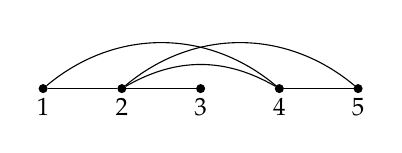
\begin{tikzpicture}
        \foreach \i in {1,2,3,4,5}{
          \node[classic] (a\i) at (\i,0) {};
          \node[below] at (a\i) {\small $\i$};
        }
        \draw (a1) -- (a2) -- (a3) (a4) -- (a5);
        \draw (a2) edge[bend left] (a4);
        \draw (a2) edge[bend left=40] (a5);
        \draw (a1) edge[bend left=40] (a4);
      \end{tikzpicture}
      \caption{A graph $G$}
    \end{subfigure}
    \hfill
    \begin{subfigure}[t]{.65\textwidth}
      \centering
      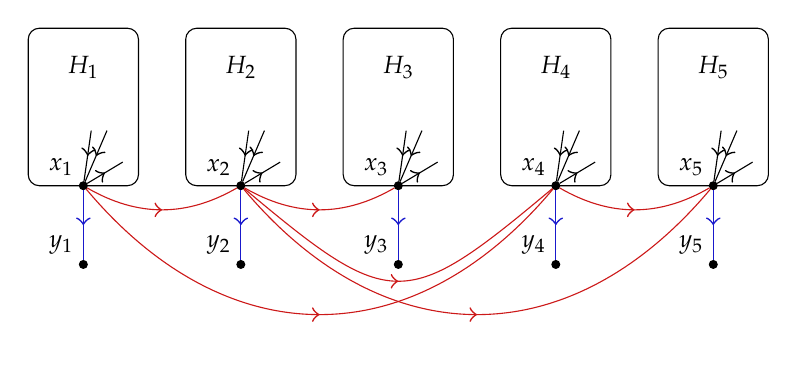
\begin{tikzpicture}[decoration={
        markings,
        mark=at position 0.5 with {\arrow[scale=1.5]{>}}}
      ]
        \foreach \i in {1,2,3,4,5}{
          \begin{scope}[shift={(2*\i,0)}]
            \draw[rounded corners] (-.2,0) rectangle (1.2,2);
            \node[classic] (x\i) at (.5,0) {};
            \node[above left] at (x\i) {\small $x_{\i}$};
            \node[classic] (y\i) at (.5,-1) {};
            \node[above left] at (y\i) {\small $y_{\i}$};
            \node (H\i) at (.5,1.5) {\small $H_{\i}$};
            \draw[postaction=decorate] (.6,.7) -- (x\i);
            \draw[postaction=decorate] (.8,.7) -- (x\i);
            \draw[postaction=decorate] (x\i) -- (1,.3);

            \draw[color3,postaction=decorate] (x\i) -- (y\i);
          \end{scope}
        }

        \draw[color1] (x1) edge[bend right,postaction=decorate] (x2);
        \draw[color1] (x2) edge[bend right,postaction=decorate] (x3);
        \draw[color1] (x4) edge[bend right,postaction=decorate] (x5);
        \draw[color1] (x2) edge[bend right=40,postaction=decorate,looseness=1.6] (x4);
        \draw[color1] (x2) edge[bend right=50,postaction=decorate,looseness=1.2] (x5);
        \draw[color1] (x1) edge[bend right=50,postaction=decorate,looseness=1.2] (x4);

      \end{tikzpicture}
      \caption{The graph $G'$ constructed. The blue arcs $x_i \to y_i$
        correspond to the vertices of $G$ and the red arcs to its edges.}
    \end{subfigure}
    \caption{Constructing an equivalent shift graph.}
    \label{fig:NP-col}
  \end{figure}

  \paragraph{Equivalence of the instances}
  Assume that there exists a 3-colouring $\alpha$ of $G$. Colour each arc
  starting in $x_u$ with the colour of $u$ in $\alpha$. At this stage it remains
  only to colour the copies of $H$. Let $\beta$ be a 3-arc-colouring of $H$. For
  each copy $H_u$, permute the colours of $\beta$ such that the arcs entering
  $x_u$ use the two colours different from $\alpha(u)$. The resulting colouring
  is a 3-arc-colouring of $G'$. Indeed, at each $x_v$, all the arcs starting in
  $x_v$ have an identical colour $\alpha(v)$, and the arcs entering $x_v$ are
  either coming from the copy $H_v$ or of the form $x_u \to x_v$ for some
  $u < v$, in both case they use colours different from $\alpha(v)$. Thus
  $L(G')$ is 3-colourable.

  Conversely, in a proper 3-arc-colouring of $G'$, by design of $H$, all the
  arcs starting in $x_u$ are coloured identically. Colour $u$ with this
  colour. Given any edge $uv$ in $E(G)$ with $u<v$, the colour of $u \in V(G)$
  is the colour of $x_u\to x_v$ which differs from the colour of $x_v \to y_v$,
  that is the colour of $v \in V(G)$. Thus $G$ is 3-colourable.

  \paragraph{$k$-iterated shift graphs}
  To adpat our reduction to $k$-iterated shift graph, we will first need to
  change our gadget. Given a $k$-iterated line digraph $G_2$ of an oriented
  graph $G_1$, we will for convenience see the $k$-colourings of $G_2$ as
  $k$-colourings of the $k$-paths of $G_1$ such that the $k$-paths
  $u_0\dots u_k$ and $u_1\dots u_{k+1}$ are coloured differently.

  For our gadget, we construct an acyclic oriented graph $H$ such that
  $\chi(L^k(H))=3$, with a marked $(k-1)$-path $X$ with the following property:
  in any 3-colouring of $L^k(H)$, the set of $k$-paths with suffix $X$ use
  exactly two colours.

  Consider the minimum $n$-vertex transitive tournament $T_n$ such that
  $\chi(L^k(T_n))=4$. For each $i \in [n]$, let $v_i$ be the vertex of indegree
  $i-1$ in $T_n$. % Let $S_n$ be the subgraph of $T_n$ obtained by removing all
  % the arcs $v_jv_{n-i}$  for all $i \in \{0, \dots, k-1\}$ and 
  % $j<n-i-1$. The oriented graph $S_n$ consists of a transitive tournament on the
  % vertices $\{v_i : i \in [n-k]\}$, with a $k$-path on the vertices
  % $v_{n-k}, \dots v_n$. Let $\phi$ be the following map from the $k$-paths of if
  % $xy\in A(S_n)$ and $\beta(uv_n) = \alpha(uv_{n-1})$ for all
  % $u \in V(T_n) \setminus \{v_{n-1},v_n\}$. The arc-colouring $\beta$ is proper
  % because $uv_n$ and $uv_{n-1}$ are twins in $L(T_n)$.  $T_n$ to the $k$-paths
  % of $S_n$. For all $k$-paths $P$ of $S_n$, $\phi(P) = P$. Any other $k$-path
  % $P$ of $T_n$ is the concatenation of a $i$-path $Q$ on the vertices of
  % $\{v_j : j < n-k\}$ and a $k-i-1$-path on vertices of
  % $\{v_j: \in \{n-k, \dots n\}$. For such paths, $\phi(P)$ is the concatenation
  % of $Q$ with $v_{n-k}, \dots v_{n-k+i-1}$. In particular, note that $P$ and
  % $P'$ are consecutive in $T_n$, \emph{i.e.} the suffix of length $k-1$ of $P$
  % is the prefix of length $k-1$ of $P'$, then $\phi(P)$ and $\phi(P')$ are
  % consecutive in $S_n$. Thus, given a colouring $\alpha$ of $L^k(S_n)$, the
  % colouring $\beta$ of $L^k(T_n)$ such that $\beta(P) = \alpha(\phi(P))$ for all
  % $P$ is a proper colouring. Since $\alpha$ and $\beta$ use the same amount of
  % colours and $S_n$ is a subgraph of $T_n$, we have
  % $\chi(L(S_n)) = \chi(L(T_n)) = 4$.
  Let $H$ be the subgraph of $T_n$ obtained by removing vertices of the form
  $v_iv_{n-k}$ with $i<n-k$ until the chromatic number of its $k$-iterated line
  digraph drops to three. Note that $S_n = T_n-\{v_iv_{n-k} : i <n-k\}$ is the
  transitive tournament on the vertices
  $v_1, \dots v_{n-k-1}, v_{n-k+1} \dots v_n$ with the additional vertex
  $v_{n-k}$ and all arcs of the form $v_{n-k}v_j$ with $j>n-k$. As such,
  $L^k(S_n)$ is isomorphic to the $k$-iterated line digraph of the transitive
  tournament on $n-1$ vertices, with one additional isolated vertex,
  corresponding to the $k$-path $v_{n-k}, \dots v_n$. So $L^k(S_n) = 3$ and $H$
  is well defined. Let $uv_{n-k}$ be the last arc removed in the construction
  of $H$, we have $\chi(L^k(H))= 3$ and $\chi(L^k(H+uv_{n-k}))=4$.

  Let $\alpha$ be a 3-colouring of $L^k(H)$, and without loss of generality
  assume that the $k$-path $v_{n-k}, \dots v_n$ is coloured 1 by $\alpha$. We
  will now argue that the set of $k$-paths with suffix $X:=v_{n-k}\dots v_{n-1}$
  is coloured with the colours 2 and 3, and thus that all the $k$-paths with
  prefix $X$ in the second part of the reduction are coloured 1. First, since
  $P=v_{n-k}\dots v_n$ is coloured 1 and is the only $k$-path starting in
  $v_{n-k}$, the $k$-paths of $H$ with suffix $X$ are coloured using a subset of
  $\{2,3\}$.

  Suppose that they all use the same colour, say 2.  Let $c$ be the colour of
  the $k$-path $uv_{n-k+1} \dots v_n$. Let $\psi$ be the map from the
  $k$-paths of $H+uv_{n-k}$ to $H$ defined as follows. For each $k$-path $P$
  avoiding the arc $uv_{n-k}$, we let $\psi(P) =P$. Given a $k$-path $P$ passing by
  $uv_{n-k}$, let $Q$ its prefix ending at $u$ and $R$ its suffix starting
  at $v_{n-k}$ and let $\psi(P)$ be the concatenation of $Q$ and
  $v_{n-k+1}, \dots v_{n-k+1+q}$ where $q$ is the length of $Q$. In particular,
  if $P$ and $P'$ are consecutive in $T_n$, then so are $\psi(P)$ and
  $\psi(P')$. Let $\beta$ be the 3-colouring of $L(H+uv_{n-k})$ defined as
  follows. For any $k$-path $P$ without $X$ as suffix or prefix, let
  $\beta(P) = \beta(\psi(P))$. Any $k$-path $P$ with suffix $X$ in
  $H+uv_{n-k}$ is either a $k$-path of $H$, in which case $\alpha(P)=2$ and we
  define $\beta(P) = 2$, or the $k$-path $uv_{n-k}\dots v_{n-1}$, in which
  case we let $\beta(P) = \alpha(uv_{n-k+1}\dots v_n) = c$. The only remaining
  $k$-path where $\beta$ is undefined is the path $P = v_{n-k} \dots v_n$ with
  $X$ as prefix. By construction the indicent paths in $L^k(H+uv_{n-k})$ are
  colored 2 and $c$, so we can colour this path with a colour from
  $\{1,3\}\setminus\{c\}$. The colouring $\beta$ is a proper 3-colouring of
  $L^k(H+uv_n)$, which contradicts $\chi(L^k(H+uv_{n-k})$. So the $k$-paths
  with suffix $X=v_{n-k}\dots v_{n-1}$ use the colours 2 and 3 in $\alpha$. To
  sum up, $L^k(H)$ is 3-colourable and in each 3-colouring of $L^k(H)$, the
  $k$-paths with prefix $X$ use two different colours.

  We finish the reduction in a similar way as for shift graphs. Let $G$ be a
  graph, with an arbitrary order on its vertices. For each vertex $u$ of $v$,
  take a copy $H_u$ of $H$ and a new vertex $y_u$, and attach an arc $x_uy_u$ to
  the last vertex $x_u$ of the marked $(k-1)$-path $X_u$ of $H_u$. For each edge
  $uv$ of $G$ with $u<v$, add a pending arc $x_uz_{uv}$ to $x_u$ and identify
  the marked $(k-1)$-path $X_v$ with the $(k-1)$-path formed by concatenating
  the suffix of length $k-2$ of $X_u$ with $z_{uv}$. As a result, the $k$-paths
  $X_ux_v$ and $X_vy_v$ are consecutive.  The oriented graph $G'$ constructed is
  acyclic because each the copies $H_u$ are acyclic and ordered following the
  order of the vertices of $G$. We consider the subgraph $L$ of $L^k(G')$
  induced by the $k$-paths that contain at most one arc between different
  vertices labelled $x_u$ for some $u$.

  We claim that $L$ is 3-colourable if and only if $G$ is 3-colourable. Let
  $\alpha$ be a 3-colouring of $G$. Let $\beta$ be the 3-colouring of $L$
  defined as follows. First, for each $u \in V(G)$, colour each $k$-path of $G'$
  with penultimate vertex equal to $x_u$ with the colour $\alpha(u)$. Each
  remaining $k$-path of $L$ is fully contained in some $H_u$ for some $u$
  because we removed from $L$ the $k$-paths containing more than one arc between
  different vertices labelled $x_u$ for some $u$. For each $u$, all the
  $k$-paths with suffix $X_u$ of $H_u$ are identically coloured, so one can
  permute the colours in a fixed 3-colouring of $L^k(H)$ to colour
  $L^k(H_u)$. Two consecutive $k$-paths of $L$ are either both contained in some
  $H_u$, or with suffix and prefix equal to some $X_u$, or with prefix equal to
  some $X_u$ and formed by the suffix of length $k-2$ of $X_u$ concatenated with
  $x_vy_v$ for some $v>u$ with $uv \in E(G)$. In either case, their colours are
  different by construction. Conversely, given a proper 3-colouring $\beta$ of
  $L$, let $\alpha$ be the colouring of $G$ such that for each $u$, $\alpha(u)$
  is the colour in $\beta$ of the $k$-path with prefix $X_u$ finishing in
  $y_u$. By design of $H$, all $k$-path with prefix $X_u$ are identically
  coloured and so $\alpha(u)$ and $\alpha(v)$ are different for each
  $uv \in E(G)$ with $u<v$, because the paths $X_ux_v$ and $X_vy_v$ are
  consecutive by construction and
  $\alpha(u) = \beta(X_ux_v) \neq \beta(X_vy_v) = \beta(v)$.
\end{proof}

We now prove that if one restricts to shift graphs of large girth (and not large
odd-girth as in \cref{thm:3col}), 3-colouring becomes a trivial problem.
\begin{theorem}
  All shift graphs of girth at least five are 3-colourable.
\end{theorem}
\begin{proof}
  Let $G$ be a shift graph of girth at least five and let $H$ be a root oriented graph
  of $G$. The vertices of $H$ have either in or out-degree at most one, because
  a vertex with in and out degree at least two produces a four-cycle in the line
  digraph. We partition the vertices of $H$ in two subsets: $X$ contains the
  vertices of indegree at most one, and $Y$ the remaining vertices, which have
  outdegree at moste one. We partition the arcs of $H$ in two subsets: $A$
  contains the arcs entering $X$ or starting in $Y$, and $B$ contains the other
  arcs, which start in $X$ and end in $Y$. The arcs of $B$ are independent so
  they can be coloured with one colour, say 1. We claim that the arcs of $A$
  form a forest, so they can be coloured with two additional colours, which
  results in a 3-arc-colouring of $H$. Let $A_1$, $A_2$ and $A_3$ the subgraphs
  formed by the arcs of $A$ that respectively connect two vertices of $X$,
  connect to vertices of $Y$, start in a vertex of $Y$ and end in a vertex of
  $X$. Because $H[X]$ has indegree at most one, the subgraph $A_1$ forms a
  forest of trees directed towards their root. Likewise, $A_2$ forms a forest of
  trees directed away their root. Because $X$ and $Y$ have respectively in and
  outdegree at most one, $A_3$ forms a matching between the roots of these two
  forests. Hence $A$ form a forest, which concludes the proof.
\end{proof}
\section{Recognising shift graphs}\label{sec:recognition}

By Schaefer's dichotomy theorem~\cite{schaefer1978Complexity}, the following
problem is NP-complete.

\begin{csproblem}{Monotone Not all equal (MNAE3SAT)}
  Given a monotone 3-CNF formula $\phi$ (in conjonctive normal form with three
  non-negated variables per clause), recognise if there exists a valuation to
  the variables such that each clause of $\phi$ contains true and false variables.
\end{csproblem}



\begin{theorem}
  Let $k \ge 1$. Recognising a $k$-iterated shift graph (or equivalently, the
  support of the $k$-iterated line digraph of
  an acyclic oriented graph) is an NP-complete problem.
\end{theorem}
\begin{proof}
  We reduce \textsc{MNAE3SAT} to the shift graph recognition problem.  Let
  $\phi$ be a monotone 3-CNF formula with $m$ clauses. We build a graph $G_\phi$
  that is a $k$-iterated shift graph if $\phi$ is a valid instance of
  \textsc{MNAE3SAT}, but is not a shift graph (and \emph{a fortiori} not a
  $k$-iterated shift graph) if $\phi$ is not a valid instance of
  \textsc{MNAE3SAT}.

  \paragraph{Gadgets}
  We first describe the gadget used for the variables. Let $H$ be the 4-sun,
  that is the graph on eight vertices composed of a 4-cycle with one pending
  edge attached to each of the vertices of the cycle. For each variable $x$,
  consider the gadget composed of a path on $8m+3$ vertices
  $u_x^{-2}, \dots, u_x^{8m}$ in which for each $i \in \{0, \ldots, 2(m-1)\}$ we
  connect each $u_x^{2i}$ to a vertex $v_x^{2i}$ itself adjacent to $w_x^{2i}$,
  and each $u_x^{2i}$ to a distinct copy of $H$ via one of the vertices of
  degree three that we will call $t_x^{2i}$ (see
  \cref{fig:variable_gadget}). For each variable $x$, denote $H_x$ the copy of
  this gadget.
  \begin{figure}[h!]
    \centering
    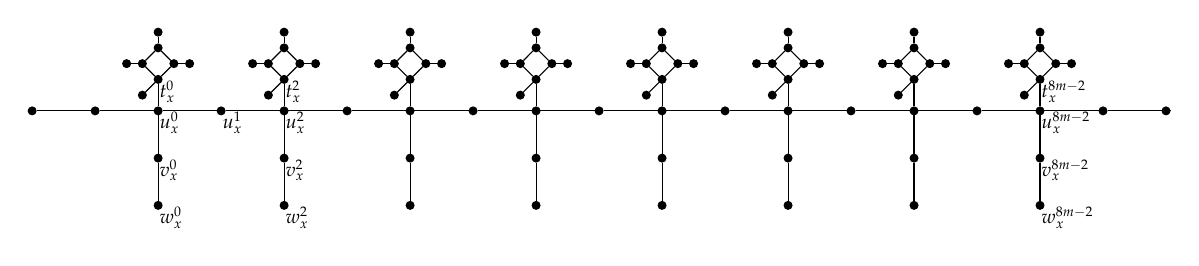
\begin{tikzpicture}[scale = .8]
      \foreach \i in {0,...,7}{
        \begin{scope}[shift={(2*\i,0)}]
          \node[classic] (a\i) at (0,0) {};
          
          \node[classic] (e\i1) at (0,-.75) {};
          \node[classic] (e\i2) at (0,-1.5) {};

          \node[classic] (H\i11) at (0,.5) {};
          \node[classic] (H\i12) at (-.25,.25) {};
          \node[classic] (H\i21) at (.25,.75) {};
          \node[classic] (H\i22) at (.5,.75) {};
          \node[classic] (H\i31) at (0,1) {};
          \node[classic] (H\i32) at (0,1.25) {};
          \node[classic] (H\i41) at (-.25,.75) {};
          \node[classic] (H\i42) at (-.5,.75) {};
          \draw (H\i11) -- (H\i21) -- (H\i31) -- (H\i41) -- (H\i11);
          \draw (H\i11) -- (a\i) -- (e\i1) -- (e\i2) ;
          \foreach \j in {1,...,4}{
            \draw (H\i\j1) -- (H\i\j2);
          }
          
        \end{scope}        
        
      }


      \node[classic] (a) at (-2,0) {};
      \node[classic] (b) at (-1,0) {};
      \node[classic] (a8) at (16,0) {};

      \draw (a) -- (b) -- (a0);

      \foreach \i in {0,...,7}{
        \node[classic] (b\i) at (2*\i+1,0) {};
        \pgfmathsetmacro{\j}{\i+1}
        \draw (a\i) -- (b\i) -- (a\j);
      }
      
      
      \node[below right=-.15cm] at (H011) {\scriptsize $t_x^0$};
      \node[below right=-.15cm] at (a0) {\scriptsize $u_x^0$};
      \node[below right=-.15cm] at (e01) {\scriptsize $v_x^0$};
      \node[below right=-.15cm] at (e02) {\scriptsize $w_x^0$};
      \node[below right=-.15cm] at (H111) {\scriptsize $t_x^2$};
      \node[below right=-.15cm] at (a1) {\scriptsize $u_x^2$};
      \node[below right=-.15cm] at (b0) {\scriptsize $u_x^1$};
      \node[below right=-.15cm] at (e11) {\scriptsize $v_x^2$};
      \node[below right=-.15cm] at (e12) {\scriptsize $w_x^2$};
      \node[below right=-.15cm] at (H711) {\scriptsize $t_x^{8m-2}$};
      \node[below right=-.15cm] at (a7) {\scriptsize $u_x^{8m-2}$};
      \node[below right=-.15cm] at (e71) {\scriptsize $v_x^{8m-2}$};
      \node[below right=-.15cm] at (e72) {\scriptsize $w_x^{8m-2}$};
    \end{tikzpicture}  
    \caption{Variable gadget $H_x$}
    \label{fig:variable_gadget}    
  \end{figure}
  
  For each $i \in \{0, \ldots, m-1\}$, we attach the gadgets $H_x$, $H_y$ and $H_z$
  of the variables appearing in the $i$-th clause $C_i = (x \vee y \vee z)$ as
  follows. Add three edges to form a path $a_ib_ic_id_i$, where $a_i=w_x^{8i}$,
  $b_i=w_y^{8i+2}$, $c_i=w_y^{8i+6}$ and $d_i=w_z^{8i}$. Denote $G_\phi$ the
  constructed graph.

  \paragraph{Valid orientations of $G_\phi$}
  We will say that an orientation of a graph is \emph{valid} if it forms a line
  digraph of an acyclic oriented graph. Before proving that there is a valuation such that
  $\phi$ has true and false variables in each clause if and only if $G_\phi$
  admits a valid orientation, we prove several lemmas describing valid
  orientations of $G_\phi$ and some of its subgraphs.

  \begin{claim}\label{cl:sun_orientation}
    There are only two valid orientations of the 4-sun, which are opposite (see
    ~\cref{fig:sun_orientation}). In these orientations, the 4-cycle is
    alternating and all vertices of degree three are transitive.
  \end{claim}
  \begin{figure}[ht]
    \centering
    \begin{tikzpicture}[decoration={
        markings,
        mark=at position 0.5 with {\arrow[scale=1.5]{>}}}
      ]
      
      \node[classic] (a) at (0,0) {};
      \node[classic] (a') at (-1,0) {};
      \node[classic] (b) at (1,1) {};
      \node[classic] (b') at (1,2) {};
      \node[classic] (c) at (2,0) {};
      \node[classic] (c') at (3,0) {};
      \node[classic] (d) at (1,-1) {};
      \node[classic] (d') at (1,-2) {};

      \draw[postaction={decorate}] (a) -- (b);
      \draw[postaction={decorate}] (c) -- (b);
      \draw[postaction={decorate}] (a) -- (d);
      \draw[postaction={decorate}] (c) -- (d);

      \draw[postaction={decorate}] (a') -- (a);
      \draw[postaction={decorate}] (b) -- (b');
      \draw[postaction={decorate}] (c') -- (c);
      \draw[postaction={decorate}] (d) -- (d');

    \end{tikzpicture}
    \caption{The only valid orientation of the 4-sun (and its opposite).}
    \label{fig:sun_orientation}
  \end{figure}
  \begin{poc}
    Let $D$ be an oriented graph with a valid orientation and whose support is the
    4-sun. By~\cref{lem:valid}, the 4-cycle $C$ of $D$ is alternating at each
    vertex. Let $v$ a vertex of degree three. Without loss of generality, assume
    that $v$ has two out-neighbours in $C$. Let $u$ be the remaining neighbour
    of $v$, and $w$ and $x$ be two vertices of $C$ such that $w$ is adjacent to
    $v$, while $x$ is not. So $D$ contains the arcs $v \to w$ and $x \to
    w$. Since $D$ is the line digraph of a graph, by the first condition
    of~\cref{lem:forbidden_config}, the edge between $u$ and $v$ is oriented
    towards $v$, hence $v$ is transitive and $D$ is of the form depicted
    on~\cref{fig:sun_orientation}.
  \end{poc}


  For each variable $x$, denote $A_x$ the subgraph of $H_x$ induced by
  $\bigcup_{i=0}^{4m-1} \{t_x^{2i}, u_x^{2i}, u_x^{2i+1}, v_x^{2i}, w_x^{2i}\}$.

  \begin{claim}\label{cl:gadget_orientation}
   
    Consider a valid orientation of $H_x$. There are only two possible
    orientations for its restriction to $A_x$, which are opposite. If
    $w_x^0 \to v_x^0$ then for all $i$, we have $w_x^{2i} \to v_x^{2i}$ if $i$
    is even and $v_x^{2i} \to w_x^{2i}$ if $i$ is odd.
  \end{claim}
  \begin{poc}
    Without loss of generality, assume that $w_x^0 \to v_x^0$.
    By~\cref{cl:sun_orientation}, each copy of the 4-sun in $H_x$ is oriented
    such that all the vertices of degree three are transitive (however,
    each copy of the 4-sun may be oriented in any of its two opposite
    orientations independently of any other copy).

    Let $i \in \{0,\ldots,4m-1\}$ and assume that $t^{2i}_x \to u^{2i}_x$
    (respectively $u^{2i}_x \to t^{2i}_x$). By \cref{cl:sun_orientation},
    $t^{2i}_x$ is transitive in the copy of the 4-sun it belongs
    to, so $t^{2i}_x$ has an outneighbour (resp. an inneighbour). Therefore,
    $u^{2i+1}_x$, $u^{2i-1}_x$ and $v^{2i}_x$ are all outneighbours of
    $u^{2i}_x$ (resp. inneighbours). As $v^{2i}_xu^{2i}_xu^{2i+1}_x$ is an
    alternating path, we also have $v^{2i}_x \to w^{2i}_x$ and $u^{2i+1}_x \to
    u^{2i+2}_x$ (respectively $w^{2i}_x \to v^{2i}_x$ and $u^{2i+2}_x \to
    u^{2i+1}_x$). The result follows from a  straightforward induction on $i$.
  \end{poc}


  Let $D$ be the graph formed by a path of length three and four pending edges
  $e_1, \ldots, e_4$, attached to the vertices of the path. Given a valid
  orientation of $D$, we say that $e_1$ and $e_4$ (respectively $e_2$ and $e_3$)
  are \emph{positive} if they are oriented away (resp. towards) the path, and
  that they are \emph{negative} otherwise.
  
  \begin{claim}\label{cl:clause_orientation}
    In any valid orientation of $D$, the edges $e_i$ cannot be all positive, or
    all negative. Conversely, any orientation of the edges $e_i$ such that $e_2$
    and $e_3$ are both positive (or both negative), and the edges $e_i$ are not
    all positive (or respectively all negative) can be extended onto $D$ into a
    valid orientation.
  \end{claim}
  \begin{poc}
    Assume that there exists a valid orientation of $D$ with all edges $e_i$
    positive. Label $a,b,c,d$ the internal vertices of $D$. Without loss of
    generality, assume that $b \to c$. As $c$ has both an inneighbour and an
    outneighbour, the edge $ab$ is oriented $a \to b$. Hence $b$ has also an
    inneighbour and an outneighbour and $e_1$ is negative. By the symmetry, if
    we had $c \to b$, $e_4$ would be negative.

    Conversely, consider an orientation of $e_1, \ldots, e_4$, such that $e_2$
    and $e_3$ are say positive, but not all four edges are positive. Say without
    loss of generality $e_1$ is negative. Then orienting $D$ as on picture
    \cref{fig:variable_gadget} forms a line digraph by
    \cref{lem:forbidden_config}.

    \begin{figure}[h!]
      \centering
      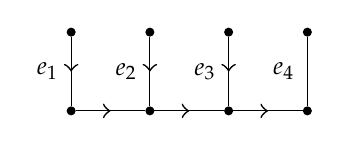
\begin{tikzpicture}[decoration={
        markings,
        mark=at position 0.5 with {\arrow[scale=1.5]{>}}}
      ]
        \foreach \i in {1,...,4}{
          \node[classic] (a\i) at (\i,0) {};
          \node[classic] (b\i) at (\i,1) {};
          \node at (\i-.3,.5) {\small $e_\i$};
        }
        
        \draw[postaction={decorate}] (a1) -- (a2);
        \draw[postaction={decorate}] (a2) -- (a3);
        \draw[postaction={decorate}] (a3) -- (a4);
        
      \draw[postaction={decorate}] (b1) -- (a1);
      \draw[postaction={decorate}] (b2) -- (a2);
      \draw[postaction={decorate}] (b3) -- (a3);
      \draw (b4) -- (a4);
          
      \end{tikzpicture}
      \caption{A valid orientation of $D$. The edge $e_1$ is negative, $e_2$ and
        $e_3$ are negative, and $e_4$ can eihter be positive or negative.}
      \label{fig:variable_gadget}
    \end{figure}
  \end{poc}

  \paragraph{Equivalence of the instances}
  We are now ready to prove that $\phi$ admits a valuation such that each
  clause contains true and false variables with different values if and only if
  $G_\phi$ is a shift graph.

  We first prove the direct implication. Consider such a valuation. For all
  variable $x$ choose the orientation of $H_x$ such that $w^{0}_x \to v^{0}_x$
  (by \cref{cl:gadget_orientation} there exists only one such orientation). The
  only edges that remain to be oriented are the edges forming the path in each
  clause gadget. Let $C_i$ be a clause of $\phi$, $D_i$ the corresponding
  subgraph of $G_\phi$, with $e_1,\ldots, e_4$ the edges attached to the vertices
  of the path of length three. By construction and \cref{cl:gadget_orientation},
  $e_2$ and $e_3$ are either both negative or both positive. Since $C_i$
  contains true and false variables, we can apply \cref{cl:clause_orientation}
  to orient the remaining edges of $D_i$. The orientation we constructed is
  valid when restricted to each $D_i$ and to each $H_x$. To check that is forms
  a valid orientation of $G_\phi$, we only need to check the first condition of
  \cref{lem:forbidden_config} at the junctions between the clause and the
  variable gadgets, and the orientation of the cycles using these
  junctions. Note that any such cycle must pass by some $u^{2i}_x$, at which it
  alternates. Finally, as each $u^{2i}_xv^{2i}_xw^{2i}_x$ forms a
  non-alternating path, the first condition of \cref{lem:forbidden_config} is
  satisfied and the orientation of $G_\phi$ is that of an acyclic line
  digraph. In other words, $G_\phi$ is a shift graph.

  We now prove the reverse implication. Consider a valid orientation of
  $G_\phi$. For each variable $x$, assign $x$ to true if $w^{0}_x \to v^0_x$ and
  to false otherwise. Let $C_i$ be a clause of $\phi$ and $D_i$ the
  corresponding variable gadget. By construction and by
  \cref{cl:gadget_orientation}, each of the edges $e_1, \ldots, e_4$ attached to
  the internal vertices of $D_i$ is positive if and only if the corresponding
  variable is true. By \cref{cl:clause_orientation}, the edges $e_1, \ldots, e_4$
  cannot be all positive or all negative because the orientation is valid. Hence
  $C_i$ contains a true and a false variable, which concludes the proof.
\end{proof}


\section*{Acknowledgements}
The research was initiated during a one-week research visit by Nicolas Trotignon
at Jagiellonian University in January 2025, supported by the grant FILL.

\nocite{*}
\bibliographystyle{abbrv}
\bibliography{references}

% \appendix
% \section{Code use for the computer check of \cref{thm:3col}}\label{sec:computer_check}
% To check that all 3-arc-colourings of $H$ colour the two arcs entering $x$ with
% different colours, we compute the number of 3-colourings of $L(H)$ and the
% number of 3-colourings of $G$, where $G$ is obtained from $L(H)$ by
% adding an edge betwenn the vertices correspoding to arcs entering $x$ in
% $H$. The following code shows that these numbers are equal, so all 3-colourings
% of $L(H)$ are 3-colourings of $G$, which implies the desired result.
% \begin{lstlisting}[language=Python]
% from sage.graphs.graph_coloring import chromatic_number, number_of_n_colorings

% # Constructing L(H)
% vertices = [(i,j) for i in range(7) for j in range(i+1,7) if j-i <= 4]
% for i in [3,4]:
%     vertices.append((i,7))
% for i in [5,6]:
%     vertices.append((i,9))  # the vertex x of H is labelled 9 here
% for i in [4,5,6]:
%     vertices.append((i,8))
% d =dict()
% for u in vertices: 
%     L = [v for v in vertices if (v[1] == u[0] or v[0] == u[1])] 
%     d[u] = L
% LH = Graph(d)

% # Computing the number of 3-colourings
% print("L(H) has " + str(number_of_n_colorings(LH,3)) + " proper 3-colourings")
% LH.add_edge((6,9),(5,9)) # LH is now the graph G
% print("G has " + str(number_of_n_colorings(LH,3)) + " proper 3-colourings")
% \end{lstlisting}

\end{document}

